%% Beginning of file 'sample631.tex'
%%
%% Modified 2021 March
%%
%% This is a sample manuscript marked up using the
%% AASTeX v6.31 LaTeX 2e macros.
%%
%% AASTeX is now based on Alexey Vikhlinin's emulateapj.cls 
%% (Copyright 2000-2015).  See the classfile for details.

%% AASTeX requires revtex4-1.cls and other external packages such as
%% latexsym, graphicx, amssymb, longtable, and epsf.  Note that as of 
%% Oct 2020, APS now uses revtex4.2e for its journals but remember that 
%% AASTeX v6+ still uses v4.1. All of these external packages should 
%% already be present in the modern TeX distributions but not always.
%% For example, revtex4.1 seems to be missing in the linux version of
%% TexLive 2020. One should be able to get all packages from www.ctan.org.
%% In particular, revtex v4.1 can be found at 
%% https://www.ctan.org/pkg/revtex4-1.

%% The first piece of markup in an AASTeX v6.x document is the \documentclass
%% command. LaTeX will ignore any data that comes before this command. The 
%% documentclass can take an optional argument to modify the output style.
%% The command below calls the preprint style which will produce a tightly 
%% typeset, one-column, single-spaced document.  It is the default and thus
%% does not need to be explicitly stated.
%%
%% using aastex version 6.3
\documentclass[linenumbers,tighten,trackchanges,twocolumn]{aastex631}

%% The default is a single spaced, 10 point font, single spaced article.
%% There are 5 other style options available via an optional argument. They
%% can be invoked like this:
%%
%% \documentclass[arguments]{aastex631}
%% 
%% where the layout options are:
%%
%%  twocolumn   : two text columns, 10 point font, single spaced article.
%%                This is the most compact and represent the final published
%%                derived PDF copy of the accepted manuscript from the publisher
%%  manuscript  : one text column, 12 point font, double spaced article.
%%  preprint    : one text column, 12 point font, single spaced article.  
%%  preprint2   : two text columns, 12 point font, single spaced article.
%%  modern      : a stylish, single text column, 12 point font, article with
%% 		  wider left and right margins. This uses the Daniel
%% 		  Foreman-Mackey and David Hogg design.
%%  RNAAS       : Supresses an abstract. Originally for RNAAS manuscripts 
%%                but now that abstracts are required this is obsolete for
%%                AAS Journals. Authors might need it for other reasons. DO NOT
%%                use \begin{abstract} and \end{abstract} with this style.
%%
%% Note that you can submit to the AAS Journals in any of these 6 styles.
%%
%% There are other optional arguments one can invoke to allow other stylistic
%% actions. The available options are:
%%
%%   astrosymb    : Loads Astrosymb font and define \astrocommands. 
%%   tighten      : Makes baselineskip slightly smaller, only works with 
%%                  the twocolumn substyle.
%%   times        : uses times font instead of the default
%%   linenumbers  : turn on lineno package.
%%   trackchanges : required to see the revision mark up and print its output
%%   longauthor   : Do not use the more compressed footnote style (default) for 
%%                  the author/collaboration/affiliations. Instead print all
%%                  affiliation information after each name. Creates a much 
%%                  longer author list but may be desirable for short 
%%                  author papers.
%% twocolappendix : make 2 column appendix.
%%   anonymous    : Do not show the authors, affiliations and acknowledgments 
%%                  for dual anonymous review.
%%
%% these can be used in any combination, e.g.
%%
%% \documentclass[twocolumn,linenumbers,trackchanges]{aastex631}
%%
%% AASTeX v6.* now includes \hyperref support. While we have built in specific
%% defaults into the classfile you can manually override them with the
%% \hypersetup command. For example,
%%
%% \hypersetup{linkcolor=red,citecolor=green,filecolor=cyan,urlcolor=magenta}
%%
%% will change the color of the internal links to red, the links to the
%% bibliography to green, the file links to cyan, and the external links to
%% magenta. Additional information on \hyperref options can be found here:
%% https://www.tug.org/applications/hyperref/manual.html#x1-40003
%%
%% Note that in v6.3 "bookmarks" has been changed to "true" in hyperref
%% to improve the accessibility of the compiled pdf file.
%%
%% If you want to create your own macros, you can do so
%% using \newcommand. Your macros should appear before
%% the \begin{document} command.
%%
\usepackage{xspace}
\usepackage{xcolor}
\usepackage{amsmath}
\usepackage{longtable}

\newcommand{\taucz}{$\tau_\mathrm{cz}$\xspace}
\newcommand{\rocrit}{$\mathrm{Ro_{crit}}$\xspace}
\newcommand{\rocritfinal}{$\mathrm{Ro_{crit}}~\lesssim~2$\xspace}
\newcommand{\lamostkep}{LAMOST--Kepler\xspace}
\newcommand{\lamostmcq}{LAMOST--McQuillan\xspace}
\newcommand{\teffmin}{5800~K\xspace}
\newcommand{\agerange}{$\sim$2--6~Gyr\xspace}
\newcommand{\agemin}{$\sim$2--3~Gyr\xspace}

\newcommand{\vdag}{(v)^\dagger}
\newcommand\aastex{AAS\TeX}
\newcommand\latex{La\TeX}

\newcommand{\rhk}{$R'_\mathrm{HK}$\xspace}
\newcommand{\shk}{$S_\mathrm{HK}$\xspace}
\newcommand{\caiihk}{Ca II H\&K \xspace}

\newcommand{\Mstar}{\ensuremath{M_{\star}}\xspace}
\newcommand{\Rstar}{\ensuremath{R_{\star}}\xspace} 
\newcommand{\Lstar}{\ensuremath{L_{\star}}\xspace} 
\newcommand{\teff}{\ensuremath{T_{\mathrm{eff}}}\xspace}  
\newcommand{\logg}{\ensuremath{\log g}\xspace} 
\newcommand{\feh}{[Fe/H]\xspace}
\newcommand{\vsini}{\ensuremath{v \sin i}\xspace} 
\newcommand{\msun}{$M_\odot$\xspace}
\newcommand{\rsun}{$R_\odot$\xspace}
\newcommand{\lsun}{$L_\odot$\xspace}
\newcommand{\tsun}{$T_\mathrm{eff,\odot}$\xspace}
\newcommand{\rhosun}{$\rho_\odot$\xspace}
\newcommand{\mstar}{$M_*$\xspace}
\newcommand{\rstar}{$R_*$\xspace}
\newcommand{\lstar}{$L_*$\xspace}
\newcommand{\rhostar}{$\rho_*$\xspace}
\newcommand{\logage}{$\text{log(age)}$\xspace}
\newcommand{\mearth}{$M_\oplus$\xspace}
\newcommand{\rearth}{$R_\oplus$\xspace}
\newcommand{\prot}{\ensuremath{P_\mathrm{rot}}\xspace}
\newcommand{\rvar}{\ensuremath{R_\mathrm{var}}\xspace}
\newcommand{\rper}{\ensuremath{R_\mathrm{per}}\xspace}

\newcommand{\gaia}{\textit{Gaia}\xspace}
\newcommand{\kepler}{\textit{Kepler}\xspace}
\newcommand{\spitzer}{\textit{Spitzer}}
\newcommand{\tess}{\textit{TESS}\xspace}
\newcommand{\emcee}{\texttt{emcee}\xspace}
\newcommand{\stardate}{\texttt{stardate}\xspace}
\newcommand{\python}{\textsc{python}\xspace}

\newcommand{\cca}{Center for Computational Astrophysics, Flatiron Institute, New York, NY 10010, USA}
\newcommand{\amnh}{Department of Astrophysics, American Museum of Natural History, Central Park West at 79th Street, New York, NY 10024, USA}
\newcommand{\columbia}{Department of Astronomy, Columbia University, 550 West 120th Street, New York, NY, USA}
\newcommand{\ifa}{Institute for Astronomy, University of Hawai’i, Honolulu, HI, USA}


%% Reintroduced the \received and \accepted commands from AASTeX v5.2
\received{\today}
\revised{\today}
%\accepted{\today}

%% Command to document which AAS Journal the manuscript was submitted to.
%% Adds "Submitted to " the argument.
%\submitjournal{PSJ}

%% For manuscript that include authors in collaborations, AASTeX v6.31
%% builds on the \collaboration command to allow greater freedom to 
%% keep the traditional author+affiliation information but only show
%% subsets. The \collaboration command now must appear AFTER the group
%% of authors in the collaboration and it takes TWO arguments. The last
%% is still the collaboration identifier. The text given in this
%% argument is what will be shown in the manuscript. The first argument
%% is the number of author above the \collaboration command to show with
%% the collaboration text. If there are authors that are not part of any
%% collaboration the \nocollaboration command is used. This command takes
%% one argument which is also the number of authors above to show. A
%% dashed line is shown to indicate no collaboration. This example manuscript
%% shows how these commands work to display specific set of authors 
%% on the front page.
%%
%% For manuscript without any need to use \collaboration the 
%% \AuthorCollaborationLimit command from v6.2 can still be used to 
%% show a subset of authors.
%
%\AuthorCollaborationLimit=2
%
%% will only show Schwarz & Muench on the front page of the manuscript
%% (assuming the \collaboration and \nocollaboration commands are
%% commented out).
%%
%% Note that all of the author will be shown in the published article.
%% This feature is meant to be used prior to acceptance to make the
%% front end of a long author article more manageable. Please do not use
%% this functionality for manuscripts with less than 20 authors. Conversely,
%% please do use this when the number of authors exceeds 40.
%%
%% Use \allauthors at the manuscript end to show the full author list.
%% This command should only be used with \AuthorCollaborationLimit is used.

%% The following command can be used to set the latex table counters.  It
%% is needed in this document because it uses a mix of latex tabular and
%% AASTeX deluxetables.  In general it should not be needed.
%\setcounter{table}{1}

%%%%%%%%%%%%%%%%%%%%%%%%%%%%%%%%%%%%%%%%%%%%%%%%%%%%%%%%%%%%%%%%%%%%%%%%%%%%%%%%
%%
%% The following section outlines numerous optional output that
%% can be displayed in the front matter or as running meta-data.
%%
%% If you wish, you may supply running head information, although
%% this information may be modified by the editorial offices.
\shorttitle{The Rossby Ridge}
\shortauthors{David et al.}
%%
%% You can add a light gray and diagonal water-mark to the first page 
%% with this command:
%% \watermark{text}
%% where "text", e.g. DRAFT, is the text to appear.  If the text is 
%% long you can control the water-mark size with:
%% \setwatermarkfontsize{dimension}
%% where dimension is any recognized LaTeX dimension, e.g. pt, in, etc.
%%
%%%%%%%%%%%%%%%%%%%%%%%%%%%%%%%%%%%%%%%%%%%%%%%%%%%%%%%%%%%%%%%%%%%%%%%%%%%%%%%%
\graphicspath{{./}{figures/}}

\begin{document}
\title{Further Evidence for Modified Spin-down in Sun-like Stars:\\Pile-ups in the Temperature--Period Distribution}

\correspondingauthor{Trevor J. David}
\email{tdavid@flatironinstitute.org}

\author[0000-0001-6534-6246]{Trevor J.\ David}
\affil{\cca}
\affil{\amnh}

\author[0000-0003-4540-5661]{Ruth Angus}
\affil{\amnh}
\affil{\cca}
\affil{\columbia}

\author[0000-0002-2792-134X]{Jason L.~Curtis}
\affil{\columbia}

\author[0000-0002-4284-8638]{Jennifer L.~van Saders}
\affil{\ifa}

\author[0000-0002-3011-4784]{Gabriella Contardo}
\affil{\cca}

\author[0000-0003-4769-3273]{Yuxi Lu}
\affil{\columbia}
\affil{\amnh}

\author[0000-0002-7550-7151]{Joel C.~Zinn}
\affil{\amnh}


\begin{abstract}
We combine stellar surface rotation periods determined from NASA's Kepler mission with spectroscopic parameters from the California-Kepler Survey and LAMOST survey to demonstrate the existence of a pile-up at the long-period edge of the effective temperature--rotation period distribution of main-sequence stars with temperatures exceeding $\sim$\teffmin. Stars in the long-period pile-up are found to have a wide range of ages (\agerange), meaning that, along the pile-up, rotation period is strongly predictive of a star's surface temperature but only weakly predictive of its age. In the effective temperature range of 5000--6250~K the long-period edge is well-described by a curve of constant Rossby number, with a critical value of \rocritfinal. The long-period pile-up was previously predicted by \citet{vanSaders2019} as a consequence of weakened magnetic braking, in which wind-driven angular momentum losses cease once stars reach a critical Rossby number. These results imply that surface rotation periods have limited predictive power for the age determination of F- and early G-type stars older than \agemin. Using kernel density estimation, we additionally detect a secondary pile-up associated with the short-period edge of the joint temperature–period distribution, which is also well-described by a curve of constant Rossby number. The short-period pile-up is not a prediction of the weakened magnetic braking hypothesis, but may instead be related to a phase of slowed surface spin-down due to core–envelope coupling previously proposed by \citet{Curtis2020} to explain the overlapping rotation sequences of low-mass members of differently aged open clusters. The relative dearth of stars with intermediate rotation periods between the short- and long-period pile-ups is also well-described by a curve of constant Rossby number, which aligns with the period gap initially discovered by \citet{McQuillan2013b} in M-type stars. These observations provide further support for the hypothesis that the period gap is due to stellar astrophysics, rather than a non-uniform star-formation history in the Kepler field.
\end{abstract}

\keywords{Stellar rotation (1629) --- Solar analogs (1941) --- Stellar evolution (1599) --- Stellar magnetic fields (1610) --- Stellar winds (1636)}

\section{Introduction} \label{sec:intro}
Solar-type and low-mass stars ($M\lesssim1.3$~\msun) lose mass and angular momentum through magnetized winds \citep{Parker1958, WeberDavis1967, Mestel1968, Kawaler1988}. Consequently, stellar rotation rates are observed to decline with age. \citet{Skumanich1972} presented the first attempt to calibrate this age-rotation relationship using the rotation periods of Sun-like stars in open clusters with independently determined ages, finding a $P_\mathrm{rot} \propto t^{1/2}$ scaling, where $t$ is stellar age. In the intervening decades, observational determinations of stellar rotation periods among open cluster members revealed how stellar spin rates evolve in more detail, leading to the calibration of the so-called gyrochronology method \citep{Barnes2003, Barnes2007, Barnes2010, MamajekHillenbrand2008, Meibom2009}.

The arrival of continuous, high-precision, long-baseline photometry from NASA's Kepler space telescope \citep{Borucki2010} provided a watershed moment for stellar rotation studies, yielding period detections for tens of thousands of stars \citep[e.g.][]{Reinhold2013, McQuillan2014, Santos2021} and allowing for gyrochronology to be extended to older ages \citep[e.g.][]{Meibom2011, Meibom2015}. NASA's subsequent K2 \citep{Howell2014} and TESS \citep{Ricker2015} missions propelled the field of stellar rotation further still, providing an exquisitely detailed picture of how spin rates evolve for stars with a broad range of masses and ages in stellar associations \citep[e.g.][]{Douglas2016, Douglas2017, Douglas2019, Rebull2016, Rebull2017, Rebull2018, Rebull2020, Curtis2019a, Curtis2019b, Curtis2020}. New and evermore precise data is becoming available at a rate that is outpacing efforts to re-calibrate gyrochronology, which is necessary to capture the complex relationship between a star's spin and its age. 

For example, efforts to calibrate gyrochronology relations using Kepler asteroseismic targets revealed tension with relations calibrated to open clusters and found that rotation periods could not be described by a single power-law relation with age \citep{Angus2015}. This tension, at least in part, is due to the fact that standard gyrochronology models are unable to account for the anomalously rapid rotation rates of stars older than the Sun, leading to the suggestion that stars with Rossby numbers of Ro~$>$~2 experience a phase of weakened magnetic braking \citep[WMB,][]{vanSaders2016}. 

Forward modeling simulations of the observed Kepler rotation period distribution also provided support for the WMB hypothesis over standard spin-down models, in that WMB models are better able to match the observed long-period edge \citep{vanSaders2019}. Those authors also predicted a pile-up of stars along the long-period edge, which they hypothesized could not be seen in the \citet{McQuillan2014} sample due to large errors on \teff in the Kepler Input Catalog \citep[KIC,][]{Brown2011}. While \citet{vanSaders2019} favored the WMB hypothesis to explain observations, those authors were also careful to point out that a long-period edge can be caused by detection biases, as stars with longer rotation periods (and larger Rossby numbers) have smaller amplitude variations which pose more difficulty to period-detection algorithms. 

More recently, \citet{Hall2021} used the asteroseismic rotation rates of Kepler dwarfs, with a different selection bias from the \citet{vanSaders2019} study and the present work, to argue support for the WMB model. \citet{Masuda2021} also found support for the WMB hypothesis from inference of the rotation period distribution of Sun-like stars using stellar radii and projected rotational velocities.  While the physics responsible for the weakened magnetic braking of solar-type stars is unknown, one hypothesis is that the declining efficiency of wind-driven angular momentum loss is connected to the magnetic field complexity, which may vary with Rossby number \citep[e.g.][]{Reville2015, vanSaders2016, Garraffo2016, Metcalfe2016, Metcalfe2019}.  

Here we examine the rotation period distribution of main-sequence stars observed by Kepler, leveraging the recent release of precise spectroscopic parameters from large-scale surveys, to demonstrate the existence of pile-ups at the long- and short-period edges of the \teff--\prot distribution of solar-type stars. We discuss our sample in \S\ref{sec:sample}, describe the steps of our analysis in \S\ref{sec:analysis}, discuss some implications of these results in \S\ref{sec:discussion}, and present our conclusions in \S\ref{sec:conclusions}.

\section{Sample Selection} \label{sec:sample}
Below, we describe the samples utilized in this work. All stars characterized here were targets of NASA's Kepler mission \citep{Borucki2010} and have published rotation periods derived from the Kepler data. For each subsample of the Kepler field described below, we combined published rotation periods from a variety of literature sources with spectroscopic parameters provided by large-scale surveys.

\begin{figure*}
    \centering
    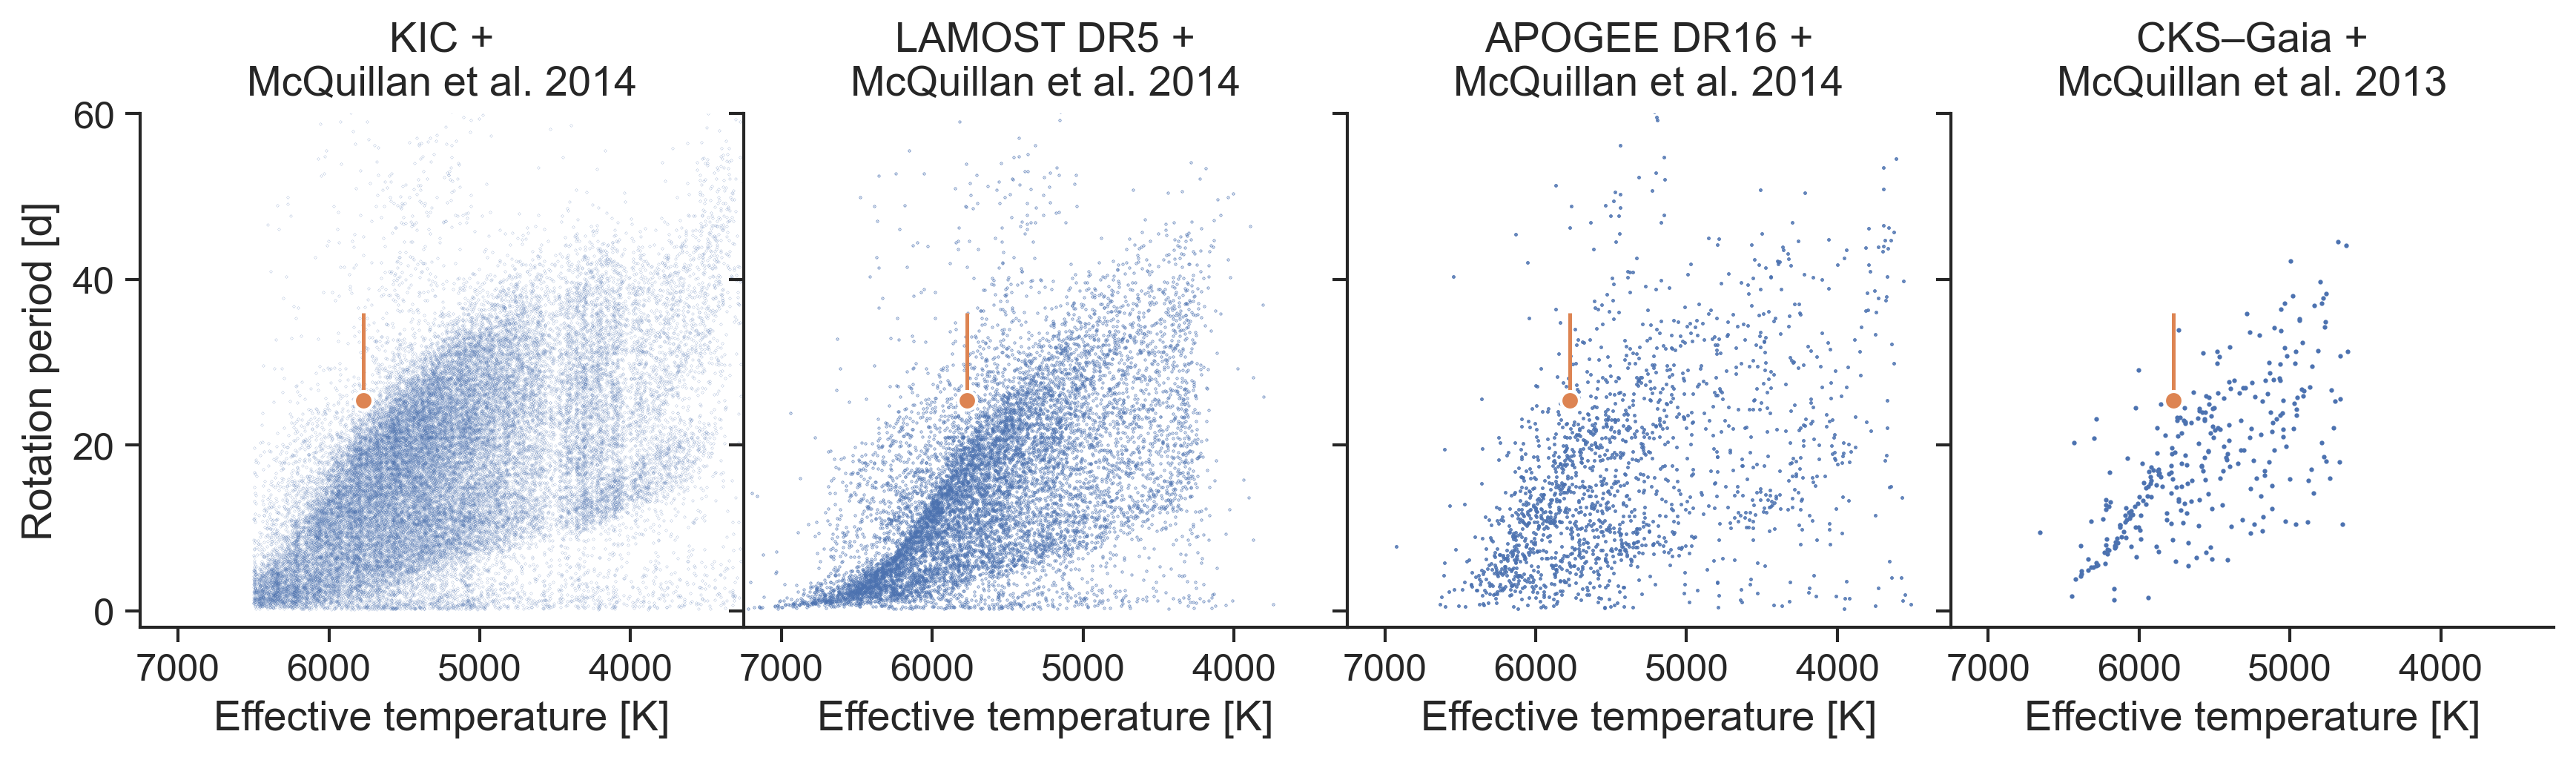
\includegraphics[width=\textwidth]{./figures/surveys.pdf}
    \caption{The \teff-\prot plane using rotation periods from \citet{McQuillan2014} or, in the case of the CKS sample, \citet{McQuillan2013} which applied an identical analysis to Kepler Objects of Interest (KOIs), with \teff originating from the source denoted at top. The \citet{McQuillan2014} \teff values originate from the Kepler Input Catalog \citep[KIC,][]{Brown2011} or \citet{Dressing2013} for low-mass stars. The orange point in each panel indicates the Sun's equatorial rotation period, with the errorbar capturing the range of periods measured from the differentially rotating surface. Many of the stars above the long-period pile-up are subgiants which have experienced spin-down due to expansion off the main-sequence, as pointed out in \citet{vanSaders2019}.}
    \label{fig:surveys}
\end{figure*}

\subsection{California--Kepler Survey} \label{subsec:cks}
The CKS project gathered high-resolution spectroscopy for 1305 Kepler planet host stars \citep{Petigura2017}. CKS spectra were acquired with the Keck/HIRES spectrograph \citep{Vogt1994} and spectroscopic parameters were determined by averaging parameters from the SpecMatch pipeline \citep{Petigura2015} and SME@XSEDE, a Python implementation of the Spectroscopy Made Easy pipeline \citep{Valenti1996}. The internal errors on \teff from the CKS catalog are 60~K. The metallicity distribution of the CKS sample is centered near solar, with a mean and standard deviation of +0.03~dex and 0.18~dex, respectively.

We compiled rotation periods for these stars from a variety of literature sources including \citet{McQuillan2013, Mazeh2015} and \citet{Angus2018}. For each star in the sample we then visually inspected the Kepler light curve folded on all available literature periods, as well as the first harmonics and sub-harmonics of those periods, and recorded our preferred period along with a reliability flag. Our procedure is explained in detail in \S2.1 of \citet{David2021}, and rotation period vetting sheets for each Kepler Object of Interest (KOI) are publicly available through Zenodo.\footnote{\url{http://10.0.20.161/zenodo.4645437}} The vast majority of stars in the CKS sample host small planets ($R_P < 4$~\rearth) and as such it is not expected that the host stars have experienced tidal spin-up from the planets.

In addition to the original CKS catalog, we also cross-matched our sample with the catalogs of \citet{Brewer2018} and \citet{Martinez2019}, both of which presented spectroscopic parameters for CKS stars based on independent analysis of the same spectra. The \citet{Brewer2018} study, referred to here as SPOCS, also published elemental abundances and ages from isochrone fitting for the CKS sample. We additionally cross-matched the CKS catalog with the LAMOST--Kepler catalog \citep{Xiang2019} which is described further in \S\ref{subsec:lamost}. We compare the \teff--\prot distributions of the CKS sample using \teff and rotation periods from a variety of sources in Appendix~\ref{app:teffprot}.

\subsection{LAMOST--Kepler} \label{subsec:lamost}
The LAMOST--Kepler project derived homogeneous spectroscopic parameters from low-resolution ($R\sim$~1800) LAMOST DR5 spectra for approximately 40\% of the Kepler field \citep{Zong2018, Xiang2019}. We cross-matched the LAMOST--Kepler stellar parameter catalog of \citet{Xiang2019} with the \citet{McQuillan2014} rotation period catalog, which published rotation periods for $>$34000 Kepler targets. The \citet{Xiang2019} catalog derived stellar parameters using the DD-Payne pipeline, which builds on the method of \citet{Ting2017b} by incorporating elements of the Cannon \citep{Ness2015} and uses the overlap with GALAH DR2 and APOGEE DR14 as training data. 

We matched 10844 LAMOST targets to 10650 unique Kepler IDs. For the Kepler sources with duplicate cross-matched LAMOST sources we kept the source with a brighter Gaia DR2 $G$ magnitude. We additionally selected sources with 3000~K~$<~\teff~<$~8000~K, 3~$<$~\logg~$<$~5~dex, and -2~$<$~[Fe/H]~$<$~2~dex. The final sample contains 10516 unique targets with well-determined \prot and \teff (having a median error of 24~K). The metallicity distribution of the LAMOST--McQuillan sample is centered near solar, with a mean and standard deviation of -0.1~dex and 0.26~dex, respectively. There is negligible overlap (3 stars) between our LAMOST--McQuillan sample and the CKS sample since the \citet{McQuillan2014} did not publish rotation periods for KOIs, which were the targets of the CKS project. Rotation periods for KOIs are instead published in \citet{McQuillan2013}, as discussed in \S\ref{subsec:cks}. 

\subsection{APOGEE--Kepler}
The Apache Point Observatory Galactic Evolution Experiment \citep[APOGEE;][]{Majewski2017} is a large-scale, high-resolution ($R \sim 22500$) stellar spectroscopic survey conducted at $H$-band as part of the Sloan Digital Sky Survey \citep[SDSS-IV;][]{Blanton2017}. The spectroscopic analysis pipeline for SDSS DR16 is described in \citet{Jonsson2020}. We used Gaia DR2 source IDs \citep{Gaia2016, Gaia2018} to cross-match Megan Bedell's Gaia--Kepler catalog\footnote{\url{https://gaia-kepler.fun/}} with the APOGEE DR16 catalog \citep{Ahumada2020}. Kepler IDs were then used to cross-match this table with the \citet{McQuillan2014} catalog. While the current overlap between Kepler targets and APOGEE is small compared to the LAMOST catalog, APOGEE DR17 will contain more dwarf stars and provide a better resource for studies such as ours. The focus of this work are overdensities in the \teff--\prot plane, and as these appear to be less prominent when using  APOGEE DR16 temperatures (Figure~\ref{fig:surveys}) we conclude that LAMOST and CKS provide more precise estimates of \teff and do not analyze the APOGEE sample further. 

\subsection{The Sun}
To place the Sun in the context of the long-period pile-up, we use up-to-date estimates of the Sun's effective temperature, rotation period, and age. Following the IAU 2015 Resolution B3 \citep{Prsa2016}, we take the nominal effective temperature of the Sun to be $\mathcal{T}^\mathrm{N}_\mathrm{eff,\odot} = 5772$~K. For the solar rotation period we adopt the equatorial rotation period of $P_\mathrm{eq,\odot}~\approx~25$~d with an upper error that encompasses the period of $\approx$~36~d measured near the poles from differential rotation studies \citep[][and references therein]{Thompson2003}.  The age of the Sun is assumed to be 4.567~Gyr from Pb-Pb dating of calcium-aluminum inclusions and chondrules recovered from primitive meteorites \citep[][and references therein]{Bahcall1995}.

\section{Analysis}
\label{sec:analysis}

\subsection{Initial observations}
A pile-up of stars along the long-period edge for stars with \teff~$>5800$~K was first noted when examining the \teff-\prot plane for the CKS sample, using the CKS \teff values and the vetted rotation period compilation from \citet{David2021}. Sourcing rotation periods from \citet{McQuillan2013, Mazeh2015} and \citet{Angus2018} revealed that this pile-up is still apparent when adopting periods uniformly from a single catalog (Figure~\ref{fig:ridge}). A secondary pile-up at the short-period edge is also apparent, though less pronounced, in the \teff--\prot distribution of the \lamostmcq sample. As shown in Figure~\ref{fig:kde}, This secondary pile-up is seen most clearly through applying Gaussian kernel density estimation (KDE), which was performed with the \texttt{seaborn} package \citep{seaborn}.

\begin{figure*}
    \centering
    \includegraphics[width=\linewidth]{./figures/kde.pdf}
    \caption{Gaussian kernel density estimation (blue contours) of the \teff--\prot distributions of the CKS--McQuillan, \lamostmcq, and asteroseismic \citet{Hall2021} samples, from left to right. Empirical cluster sequences from \citet{Curtis2020} are shown by the dark grey lines. The orange dashed lines show constant Rossby curves of fiducial values (see \S\ref{subsec:rossby}). The short-period pile-up can be observed in the LAMOST--McQuillan sample for \teff~$\gtrsim$~5500~K. The orange point indicates the Sun's temperature and equatorial rotation period, with the errorbar capturing the range of periods measured from its differentially rotating surface.}
    \label{fig:kde}
\end{figure*}

The location of the short-period pile-up is close to the empirical hybrid cluster sequence derived by \citet{Curtis2020} from members of the NGC~6819 (age~$\sim$~2.5~Gyr) and Ruprecht~147 (age~$\sim$~2.7~Gyr) open clusters (Figure~\ref{fig:kde}). Notably, we use the color--\teff relation presented by those authors to recast the cluster sequences in terms of \teff. As we show in \S\ref{subsec:ages}, stars along the pile-up have a range of ages. Therefore, the observation that the edge approximately corresponds with the $\sim$2.5--2.7~Gyr cluster sequence implies that stars with \teff$\lesssim 5800~K$ have already piled up onto the edge by or before this timescale. Similarly, the edge is well-separated from the empirical $\sim$1~Gyr cluster sequence based on rotation rates in the NGC~6811 cluster \citep{Curtis2020}, implying that it takes F-type stars $>1$~Gyr to converge onto the long-period edge. These observations are in accordance with predictions from the WMB model which suggest the pile-up forms on a timescale of 2--3~Gyr \citep{vanSaders2019}.

In both the CKS and LAMOST samples, there is a change of slope along the ridge, with an inflection point corresponding closely to the Kraft break at $\approx$~6250~K, the point at which convective envelopes become vanishingly thin \citep{Kraft1967}. A piecewise linear fit to the ridge in the CKS sample confirmed that the inflection point occurs at \teff~=~6250~$\pm$~32~K, where the uncertainty was estimated from Markov chain Monte Carlo (MCMC) sampling. This change in slope is likely due to the fact that the convective turnover timescale, \taucz, changes rapidly above 6250~K.

In the CKS sample, there appears to be a clustering of stars above the ridge with \teff~$>6100$~K (seen most clearly in the top panels of Figure~\ref{fig:models}). This cluster of points has a similar slope in the \teff--\prot plane as the long-period pile-up, and does not reside on the harmonic of the ridge line as one might expect if the periods were erroneously determined. After inspecting the light curves of stars on the ridge and above the ridge in the temperature range 6100~K~$<$~ \teff~$<6300$~K we did not notice any obvious trends or differences between the two samples. The periods of the stars in the cluster above the ridge appear to be just as reliable as those on the ridge. Interestingly, a similar clustering of points is not observed in the LAMOST--Kepler sample and is less pronounced or absent when substituting the CKS temperatures with \teff from either \citet{Brewer2018} or \citet{Martinez2019}, two studies that independently derived spectroscopic parameters from the CKS spectra. Further inspection of the stars in this cluster revealed that they have anomalously large \teff discrepancies between the CKS and SPOCS catalogs, such that the SPOCS temperatures shift the stars onto the long-period pile-up. We conclude that the temperatures for these stars in the CKS catalog are too high by $\gtrsim$~100~K.

\subsection{Comparison with theory}
\label{subsec:models}

We compared the \teff--\prot distribution of the CKS and LAMOST--Kepler samples with the theoretical predictions of \citet{vanSaders2019}. Those authors presented forward modeling simulations of the observed Kepler \prot distribution including theoretical models of stellar angular momentum evolution (for both the standard spin-down and WMB scenarios), a galactic population model, and a prescribed observational selection function. The theoretically predicted \teff--\prot distributions of \citet{vanSaders2019} are shown in relation to the observations in Figure~\ref{fig:models}. Neither model satisfactorily matches the observations, though the WMB model more closely matches the long-period edge of F-type and early G-type stars. The specific WMB prescription of \citet{vanSaders2019} adopted a critical Rossby number of \rocrit~=~2.08, leading to a pile-up that is located at larger \prot values (at fixed \teff) when compared to the observations. 

To quantify the degree of agreement between the theoretical models and observations we computed the 10th and 90th percentile \prot ranges of the standard and WMB models in overlapping \teff bins, analogous to how the upper and lower boundaries of the observed \prot distribution were found in \S\ref{subsec:rossby}. We computed the $\chi^2$ values between the observed upper edge and the 90th percentile ranges of the standard and WMB models, finding the WMB model is preferred with a $\Delta \chi^2 = 154$. Moreover, the WMB model better reproduces the slope of the observed long-period edge between 5300--6000~K (Figure~\ref{fig:percentiles}). 

While better agreement between the WMB model and observations might be achieved with stalling at a lower \rocrit, it is also possible that there are systematic offsets in the \teff scales between the observations and models used in \citet{vanSaders2019}, as well as differences in the computation of \taucz.  We also note that, while the models were computed using a simulated Kepler stellar population and selection function, the actual observed population and selection function of the LAMOST--Kepler catalog may be slightly different. 

Shifting the LAMOST \teff to higher values would bring the data into better agreement with the models. In turn, it appears that the long-period edge for lower mass stars would be at higher \prot than the models (i.e. the low-mass stars would be rotating more slowly than the model predictions). Such a discrepancy could result from different underlying populations between the models and the \lamostmcq sample, or a different normalization for the magnetic braking law. The models above employ a modified magnetic braking law that is scaled to match the rotation period of the Sun \citep[see equations 1 \& 2 of][]{vanSaders2013}, with a normalization factor of $f_K = 6.6$. A higher normalization factor would cause the low-mass stars to spin down more at fixed age.

Notably, both models fail to reproduce the observed short-period pile-up, possibly due to the assumption of solid-body rotation in both models. At early times, Sun-like and low-mass stars are expected to have strong radial differential rotation due to their rapid collapse onto the main-sequence. The core and envelope at these times are thus assumed to be decoupled. However, the core and envelope are expected to couple on timescales of a few tens of million years for Sun-like stars \citep{Denissenkov2010, GalletBouvier2015, Lanzafame2015} or hundreds of million years for low-mass stars \citep{GalletBouvier2015,Lanzafame2015,Somers2016}. When this happens, angular momentum can be transferred from the core to the envelope at a rate comparable to the rate at which angular momentum is lost via magnetized winds. Consequently, so-called ``two-zone'' models \citep{MacGregor1991} spin more rapidly than solid-body rotators at the same age. This hypothesis is discussed further in \S\ref{subsec:shortperiod}.

\begin{figure*}
    \centering 
    \includegraphics[width=0.49\linewidth]{./figures/std-model-cks.pdf}
    \includegraphics[width=0.49\linewidth]{./figures/wmb-model-cks.pdf}
    \includegraphics[width=0.49\linewidth]{./figures/std-model-lamost.pdf}
    \includegraphics[width=0.49\linewidth]{./figures/wmb-model-lamost.pdf}
    \caption{The \teff-\prot plane for the CKS sample (top panels) and LAMOST sample (bottom panels) in comparison to the standard and WMB models presented in \citet{vanSaders2019}. The excess of stars with periods $\gtrsim$~35 days, seen most clearly in the models, are due to subgiants which have expanded off the main-sequence \citep[referred to as the long-period overdensity in][]{vanSaders2019}. Rotation periods for the CKS sample here are sourced from the \citet{David2021} compilation.}
    \label{fig:models}
\end{figure*}

\begin{figure}
    \centering
    \includegraphics[width=\linewidth]{./figures/percentiles.pdf}
    \caption{Discrepancies between the observed and theoretically predicted \teff--\prot distribution of Kepler stars. Comparison of the 10th and 90th \prot percentiles predicted from the standard (light blue) and WMB (blue) models of \citet{vanSaders2019} with the same percentile ranges from the LAMOST--McQuillan sample (black points).}
    \label{fig:percentiles}
\end{figure}

\subsection{Comparison with asteroseismic rotation rates}
\label{subsec:asteroseismic}

\citet{Hall2021} determined rotation periods for 91 main-sequence, asteroseismic Kepler targets from rotational splitting of asteroseismic oscillation frequencies. We found that the distribution of the asteroseismic sample in the \teff--\prot plane approximately matches the pile-up we observe, although the \citet{Hall2021} sample appears shifted slightly to either higher \prot or higher \teff values relative to the ridge in the LAMOST--Kepler sample while such an offset is either absent or not as apparent relative to the CKS sample. Such an offset could be due to differing spectroscopic temperature scales between the two studies. To investigate the origin of this offset, we cross-matched the \citet{Hall2021} sample with the LAMOST DR5 catalog \citep{Xiang2019}. We found a root mean square (RMS) of the residuals between the \citet{Hall2021} and LAMOST DR5 \teff measurements of 55~K, with a median offset of 41~K, such that the LAMOST \teff scale is cooler, on average. Though this discrepancy is modest, adopting the LAMOST \teff scale appeared to resolve most of the offset between the pile-up as seen in the two samples. 

\begin{figure}
    \centering
    \includegraphics[width=\linewidth]{./figures/asteroseismic.pdf}
    \caption{Comparison of CKS (left) and LAMOST--Kepler samples (right) with the \citet{Hall2021} main-sequence asteroseismic sample in the \teff--\prot plane. Note, the CKS, LAMOST, and \citet{Hall2021} samples derive \teff from distinct pipelines. A constant offset of +41~K was applied to the LAMOST \teff to bring that sample onto the same scale as the asteroseismic sample (see Appendix~\ref{app:teff}). Using LAMOST \teff, where it exists, for the \citet{Hall2021} sample brings that sample into even closer agreement with the long-period pile-up in the LAMOST-McQuillan sample.}
    \label{fig:asteroseismic}
\end{figure}

\subsection{Constant Rossby model}
\label{subsec:rossby}
In the WMB model of \citet{vanSaders2016, vanSaders2019}, a star spins down until it reaches a critical Rossby number, at which point magnetic braking ceases. Since Rossby number is highly sensitive to temperature through its dependence on the convective turnover timescale ($\mathrm{Ro} = P_\mathrm{rot}/\tau_\mathrm{cz}$, where $\tau_\mathrm{cz}$ is the convective turnover timescale), this critical threshold corresponds to different rotation periods for stars of different \teff, leading to a pile-up in the \teff-\prot plane. Using a small sample of Kepler targets with rotation periods determined from brightness modulations, \citet{vanSaders2016} proposed this threshold happens at a critical Rossby number of $\mathrm{Ro_{crit}} \sim \mathrm{Ro_\odot}$. 

We tested the hypothesis that the long-period pile-up observed in the LAMOST--Kepler sample is due to WMB by fitting constant Rossby models to the \prot boundary. For a given \teff, this model predicts \prot as: 

\begin{equation} \label{eq:1}
    \prot (\mathrm{Ro}, \teff) = \mathrm{Ro} \times \tau_\mathrm{cz}(\teff),
\end{equation}

where we used the equation for the convective turnover timescale (valid in the \teff range of 3300~K$\lesssim \teff \lesssim$~7000~K) presented in \citet{Gunn1998} and replicated in \citet{CranmerSaar2011}:

\begin{multline} \label{eq:2}
\tau_\mathrm{cz}(\teff) = 314.24\exp \left [ -\left (\frac{T_\mathrm{eff}}{1952.5 \mathrm{K}}  \right ) - \left (\frac{T_\mathrm{eff}}{6250 \mathrm{K}}  \right )^{18} \right ] \\+ 0.002.
\end{multline}

To obtain a reasonable description of the long-period edge we computed the 90th percentile of \prot values in overlapping \teff bins with centers located every 20~K between 4000~K and 7000~K and half-widths of 100~K. We found it was also necessary to omit stars with Ro~$>$~5/3 in this computation to match the long-period edge. Since we observed a break in the 90th percentile \prot curve near \teff~=~4250~K, due to smaller sample sizes at low \teff, we restricted the analysis below to stars with \teff$>~4250$~K. To compute approximate uncertainties on the 90th percentile curve we performed 100 bootstrapped resamplings in each bin, leaving out 50\% of the data for each resampling. The 90th percentile curve and its uncertainty was then computed from the mean and standard deviation of the boostrapped values. We computed the 10th percentile curve and its uncertainty similarly, as an approximation to the lower boundary of the \teff-\prot plane. We show these curves in relation to the full LAMOST--Kepler sample and to constant Rossby models in Figure~\ref{fig:mcmc}.

We performed an initial Levenberg-Marquardt non-linear least-squares fit of a constant Rossby model to the long-period edge with the \texttt{curve\_fit} function in the \texttt{scipy.optimize} class to optimize the following likelihood: 

\begin{multline} \label{eq:3}
    \ln{p} (y | T_\mathrm{eff}, \sigma, \mathrm{Ro}, f) =\\ -\frac{1}{2}\sum_n \left [ \frac{(y_n - P_\mathrm{rot}(\mathrm{Ro}, T_\mathrm{eff} - T_\mathrm{sys}))^2}{s_n^2}  + \ln{(2\pi s_n^2)} \right ],
\end{multline}

where

\begin{equation} \label{eq:4}
    s_n^2 = \sigma^2 + f^2 P_\mathrm{rot}(\mathrm{Ro}, T_\mathrm{eff} - T_\mathrm{sys})^2,
\end{equation}


and $y_n$ is the value of a \prot percentile curve in the $n$th \teff bin. This is a Gaussian likelihood where the variance is underestimated by some fraction, $f$. Here $T_\mathrm{sys}$ is a constant to allow for a systematic offset between the data and the models used to calibrate the \taucz relation. We performed Markov chain Monte Carlo sampling (MCMC) of this likelihood with the \texttt{emcee} package \citep{emcee2013, emcee2019} to estimate the mean and uncertainty of the critical Rossby number that best matches the long-period edge in the range of 5000~K$\lesssim \teff \lesssim$~6250~K. We instantiated 32 walkers around the least-squares solution and sampled for $10^5$ steps, adopting uniform priors on Ro $f$, and $T_\mathrm{sys}$ with ranges of (0.1,10), (0,10), and (-1000~K, 1000~K), respectively. Convergence was assessed by ensuring the chain length was at least 100 times longer than the chain autocorrelation lengths for each parameter. A similar analysis was performed for the 10th percentile curve, restricted in the range of 4500~K$\lesssim \teff \lesssim$~5800~K where a constant Rossby model provides a reasonable fit. 

We additionally fit the CKS long-period pile-up (using three different homogeneous \teff sources), the \citet{Hall2021} asteroseismic main-sequence sample, and all combined data sets of the long-period pile-up, allowing for \teff offsets in each data set (Table~\ref{tab:mcmc}). For the CKS pile-up stars, the \prot uncertainties were assumed to be 1~d. To isolate the long-period pile-up stars in the CKS sample, we selected a trapezoidal region using the condition $-0.0314~\teff + 199.286 < \prot < -0.0314~\teff + 206.286$. We note that this selection is particular to the CKS \teff scale and is not general. For the CKS sample, we additionally required $\logg~>~4$ and 5850~K~$<~\teff~<$~6500~K. In the joint fit of all data sets, the log likelihood was defined as the sum of log likelihoods (given by Eq.~\ref{eq:3}) from the individual data sets.

The constant Rossby model provides a reasonably good description of the \lamostmcq long-period edge in the \teff range of $\approx$~5000--6250~K, with fractional residuals $\lesssim5\%$ over this range. Above and below this \teff range we see clear and significant divergence from the constant Rossby model, such that the model under-predicts periods of hotter stars and over-predicts periods of cooler stars, possibly because the cooler stars have not had enough time to evolve to that Rossby number \citep[see Figure 6 in][]{vanSaders2019}.

We caution that the specific values of \rocrit found here are highly sensitive to shifts in the \teff scales between the models and observations, as well as the \teff scale of the models used to derive the \taucz relation. Therefore, while we find values of \rocritfinal are able to explain the various individual data sets, a value of \rocrit  $\approx$~2 may be compatible with all of the data sets if modest \teff systematics are present. Comparison of the long-period pile-ups as seen in the CKS and \lamostmcq samples support the notion that the LAMOST \teff scale is about 30--40~K cooler than the CKS scale (see also Appendix~\ref{app:teff}).

\begin{figure}
    \centering
    \includegraphics[width=\linewidth]{./figures/mcmc.pdf}
    \caption{\textit{Top:} Gaussian kernel density estimation of the LAMOST--McQuillan sample and the 10th and 90th \prot percentiles (which and black points, respectively), computed as described in \S\ref{subsec:rossby}. \textit{Middle:} The same 10th and 90th percentile curves shown in relation to constant Rossby curves. \textit{Bottom:} Residuals from the median models resulting from the MCMC sampling. The fits depicted above do not include a \teff offset.}
    \label{fig:mcmc}
\end{figure}


\begin{deluxetable*}{lllll}
\tabletypesize{\scriptsize}
\tablecolumns{5}
\tablewidth{0pt}
\tablecaption{Results of constant Rossby model fits.\label{tab:mcmc}}
\tablehead{
\colhead{Sample} & 
\colhead{\teff range} & 
\colhead{Ro} & 
\colhead{f} & 
\colhead{$T_\mathrm{sys}$ (K)} 
}
\startdata
\textit{Short-period pile-up} \\
\hline
\lamostmcq 10th \prot pctl. & 4500~K--5800~K & 0.367 $\pm$ 0.009 & 0.008 $\pm$ 0.006 &  44 $\pm$ 36 \\
\hline 
\textit{Long-period pile-up} \\
\hline
\lamostmcq 90th \prot pctl. & 5000~K--6250~K & 1.37 $\pm$ 0.02 & 0.005 $\pm$ 0.004 & 59 $\pm$ 15 \\
\lamostmcq 90th \prot pctl. & 5800~K--6250~K & 1.41 $\pm$ 0.09 & 0.01 $\pm$ 0.01 & 42 $\pm$ 37 \\
CKS (CKS \teff) & 5800~K--6250~K & 1.75 $\pm$ 0.07 & 0.05 $\pm$ 0.01 & -58 $\pm$ 16 \\ 
CKS (SPOCS \teff) & 5800~K--6250~K & 1.9 $\pm$ 0.1 & 0.09 $\pm$ 0.01 & -123 $\pm$ 20 \\
CKS (M19 \teff) & 5800~K--6250~K & 1.6 $\pm$ 0.1 & 0.17 $\pm$ 0.02 & 26 $\pm$ 38 \\
\citet{Hall2021} main-sequence & 5000~K--6250~K & 1.7 $\pm$ 0.2 & 0.30 $\pm$ 0.04 & -5 $\pm$ 64 \\
\citet{Hall2021} main-sequence & 5800~K--6250~K & 1.9 $\pm$ 0.4 & 0.27 $\pm$ 0.05 & -29 $\pm$ 79 \\
All samples & 5000~K--6250~K & 1.47 $\pm$ 0.05 & 0.132 $\pm$ 0.008 & 2 $\pm$ 23 (LAMOST) \\
 & & & & 10 $\pm$ 15 (CKS) \\
 & & & & 61 $\pm$ 21  (Hall) \\
All samples & 5800~K--6250~K & 1.67 $\pm$ 0.08 & 0.116 $\pm$ 0.009 & -42 $\pm$ 24 (LAMOST) \\
&  &  &  & -44 $\pm$ 20 (CKS) \\
&  &  &  & 3 $\pm$ 23 (Hall) \\ 
\enddata
%\tablecomments{}
\end{deluxetable*}

\subsection{Ages of stars on the long-period pile-up}
\label{subsec:ages}
The WMB model predicts that hotter stars pile up on the long-period edge at younger ages, producing an age gradient across the edge. In Figure~\ref{fig:ages} we show the \teff-age distributions of stars on the ridge using ages from the CKS and SPOCS \citep{Brewer2018} catalogs, where we use the trapezoidal selection described in \S\ref{subsec:rossby} to select stars on the long-period pile-up. Both catalogs derive spectroscopic parameters from the CKS spectra, but use different pipelines for both the spectroscopic parameters and the isochrone fitting. In both cases, there appears to be an age gradient such that hotter stars are younger on average. However, such a trend is also expected in a sample of main-sequence stars as a natural consequence of the shorter main-sequence lifetimes of hotter, more massive stars. We also find that the dispersion in age is a sensitive function of \teff, with cooler stars on the ridge showing a broader range of ages. This observation could be due to cooler stars populating the ridge for longer periods of time (relative to hotter stars), the lower precision of isochrone ages for cooler stars, or some combination of the two effects.

We determined that 90\% of the stars on the ridge have ages between 1.4--5.6~Gyr (using ages from the CKS catalog), or 2.3--5.9~Gyr (using SPOCS ages). However, we note that systematic effects in surveys and theoretical models lead to large uncertainties in isochrone ages that are not necessarily represented by the reported age uncertainties. The SPOCS ages in particular are questionable given that only $\sim$1\% of the stars have ages $<$~2~Gyr and the concentration of stars at the upper age boundary at a given \teff (Figure~\ref{fig:ages}). In fact, there are only a handful of long-period pile-up stars in the CKS sample with ages older than the age of the Sun (using CKS ages), and almost all of the pile-up stars would be compatible with an age equal to or less than the Sun's given the large age uncertainties. 

In the WMB model, although wind-driven angular momentum losses cease, stars continue to evolve structurally which results in evolution in the moment of inertia and stellar spin, driven by expansion of the stars away from the main-sequence \citep{vanSaders2019}. As a result, an age-gradient is expected along the pile-up as stars of different mass depart the pile-up at different ages. Though we have not measured this gradient, the data suggest that some stars spend several Gyr occupying the ridge with only modest evolution of their spin rates.

We additionally selected stars on the long-period pile-up from the \lamostmcq sample by selecting stars with periods within 5\% of the Ro~=~1.3 curve (which traces the center of the highest density contour in Figure~\ref{fig:kde}) , 5500~K~$<$~\teff~$<$~6500~K, and 4~dex~$<$~\logg~$<$~4.75~dex. While ages for the \lamostkep sample are not available, the broad distribution of these stars in the spectroscopic H-R diagram supports the inference from the CKS sample that the long-period pile-up is populated by stars with a broad range of ages (Figure~\ref{fig:ages}). Interestingly, the solar \teff and \logg values appear to be wholly consistent with the distribution of long-period pile-up stars. We discuss the Sun in context of the long-period pile-up further in \S\ref{subsec:thesun}.

\begin{figure*}
    \centering
    \includegraphics[width=\linewidth]{./figures/ages.pdf}
    \caption{Above, H-R diagram placement of long-period pile-up stars relative to the Sun and the CKS sample (a) and similarly for the LAMOST--Kepler sample (b). Below, the \teff-age plane for CKS stars along the long-period pile-up using isochrone ages from the CKS (c) and SPOCS (d) catalogs.}
    \label{fig:ages}
\end{figure*}

\subsection{Where do the pile-ups end?} \label{subsec:extent}
It appears from Figures~\ref{fig:kde} and \ref{fig:models} that the number density of stars on the long- and short-period pile-ups declines towards cooler \teff. While it not clear whether or not these declines are astrophysical in nature, the result of the Kepler selection function or observational biases, or some combination of effects, we attempted to characterize the extent of the pile-ups through the following approach. We found through inspection that constant Rossby curves of Ro=0.5 and Ro=1.3 (for the short- and long-period pile-ups, respectively) appear to describe the highest density contours found from Gaussian kernel density estimation of the \lamostmcq sample. In windows of 10~K width we measured the fraction of stars with periods within 1~d of each of the two constant Rossby curves, relative to the total number of stars in that \teff window. We found that the relative fraction of stars on the long-period pile-up declines rapidly between 6500~K and 5800~K, by more than half in that temperature range before plateauing at cooler \teff (Figure~\ref{fig:fraction}). The relative fraction of stars on the short-period edge declines more slowly, and below the temperature of the Sun, the relative fractions of stars on the two pile-ups are nearly equal. Thus, it is not yet clear if either pile-up extends to temperatures cooler than \tsun.

\begin{figure}
    \centering
    \includegraphics[width=\linewidth]{./figures/fraction.pdf}
    \caption{The relative fraction of stars on the long- and short-period pile-ups, in the \lamostmcq sample, in 10~K windows of \teff.}
    \label{fig:fraction}
\end{figure}


\section{Discussion} \label{sec:discussion}

\subsection{Long-period behavior} \label{subsec:longperiod}

As discussed in \S\ref{subsec:models} and \S\ref{subsec:rossby}, the existence of a pile-up of stars with a constant Rossby number is consistent with expectations from the WMB model of \citet{vanSaders2016, vanSaders2019}. The location of the long-period pile-up coincides closely with the cluster of main-sequence stars with asteroseismic rotation rates determined by \citet{Hall2021} and we suggest the two features are one and the same. Offsets in both observational and theoretical \teff scales between different studies can explain the modest discrepancies between the asteroseismic sample and the samples considered here, as well as discrepancies in the \rocrit values inferred here and those proposed in \citet{vanSaders2019}. {\color{red} Furthermore, we note that there are important differences between the samples considered here and the \citet{Hall2021} asteroseismic sample. The present samples have rotation periods detected from photometric variations and, for a survey of finite baseline and sensitivity like Kepler, photometric rotation periods are harder to detect for slower rotators, smaller amplitude variations, and more stochastic variability patterns. Exacerbating the problem of detection, slower rotation tends to be accompanied by smaller-scale and less periodic variability. The asteroseismic sample, by comparison, is less biased and more likely to contain pile-up stars that our sample may have missed. It is evident from Figure~\ref{fig:gap} that the long-period pile-up also coincides with a steep gradient in variability amplitude, such that a hidden population of pile-up stars may lie just beyond the edge of detectability. This effect, in addition to the \teff offsets mentioned above, can further bias our inference of \rocrit to lower values. Regardless of the biases mentioned above and the true value of \rocrit, the sample considered clearly indicates that the long-period pile-up is apparent for stars with \teff~$\gtrsim$~\teffmin with Rossby numbers lower than those associated with a detection edge.}

Recently, \citet{LorenzoOliveira2019} studied the \prot--age relation of solar twins observed by the Kepler mission, finding marginal statistical evidence in favor of a standard spin-down model over the WMB model. Those authors posited that if WMB takes place for Sun-like stars, it should happen at \rocrit~$\gtrsim 2.29$ or ages~$\gtrsim$~5.3~Gyr.\footnote{A case study of an $\sim$8~Gyr solar twin further reinforced these conclusions \citep{LorenzoOliveira2020}.} By comparison, our findings provide support for the WMB model among stars that are slightly hotter than the Sun, but at \rocrit~$\lesssim$~2 and at ages in the range of $\sim$2--6~Gyr. Furthermore, we find that the long-period pile-up lies clearly below an empirical 2.5~Gyr gyrochrone of \citet{Curtis2020} that is evolved forward to 5.3~Gyr for braking indices of $n=0.5$ or $n=0.65$, which invalidates the claim of \citet{LorenzoOliveira2019}. Notably, the \citet{LorenzoOliveira2019} work did not include changes in the stellar moment of inertia in the spin-down calculations. Neglecting spin-down due to expansion will lead to more rapid rotation rates that allow standard spin-down models to match observations, leading to the erroneous conclusion that WMB is not required.

We note that the \rocrit values we found in \S\ref{subsec:rossby} are smaller than the values of $\sim$2 found by \citet{vanSaders2016,vanSaders2019}, however, these results are sensitive to different \teff scales and different prescriptions for \taucz. We explored the \taucz formulae of \citet{BarnesKim2010} and \citet{Landin2010}, but these produce larger \taucz at fixed \teff than the \citet{Gunn1998} relation, which exacerbates the \rocrit mismatch mentioned above.


\subsection{Short-period behavior} \label{subsec:shortperiod}

Unlike the long-period pile-up, the short-period pile-up is not predicted by the WMB model or, more generally, any standard, solid-body braking model. However, this feature may also be due to an epoch of apparent stalling, albeit a temporary one since cluster studies demonstrate that stars continue to spin down beyond the short-period pile-up. Works examining the \teff–\prot sequences of open clusters have found overlap between low-mass members in clusters of different ages, notably Praesepe (0.67~Gyr), NGC 752 (1~Gyr), and NGC 6811 (1.4~Gyr) \citep{Agueros2018, Curtis2019a, Curtis2020}. In other words, the spin rates of low-mass stars appear to evolve very little in the time elapsed between the ages of those clusters. The short-period pile-up we observe may be the manifestation of the same type of slowed spin evolution, but for stars of higher masses and younger ages than the cluster members in the above-mentioned works (since the pile-up is observed at shorter periods relative to the Praesepe sequence). 

\citet{Curtis2019a, Curtis2020} proposed that the overlapping cluster sequences could be produced by a temporary epoch of stalled spin-down, caused either by (i) a reduction in the magnetic braking torque, or (ii) core–envelope momentum transfer which offsets the effect of magnetic braking \citep[e.g.][]{MacGregor1991}. In the core–envelope momentum transfer scenario angular momentum is exchanged between the envelope and the core on a characteristic timescale known as the core–envelope coupling timescale. The angular momentum transfer spins up the envelope, temporarily offsetting the spin-down via magnetic braking. Thus, in the core–envelope coupling scenario, spin evolution is slowed when the star's age becomes comparable to the core–envelope coupling timescale. Theoretical predictions for the core–envelope coupling are mass-dependent, and for a solar-mass star range from 30--110 Myr \citep{Bouvier2008, IrwinBouvier2009, Denissenkov2010, GalletBouvier2015, Lanzafame2015, Somers2016, Spada2020}. 

After a period of slowed spin-evolution, stars must resume spinning down as evidenced from studies of older open clusters. From open cluster data \citet{Curtis2020} estimated that solar-mass stars resume spin-down after $\approx$~230~Myr. Thus, if core–envelope coupling is responsible for delaying the spin-down of stars, and if the theoretical core–envelope coupling timescales are accurate, then we may expect Sun-like stars to experience little spin evolution between $\sim$100~Myr and $\sim$200~Myr. This picture is compatible with open cluster studies which show multiple cluster sequences of Sun-like stars overlapping at ages of $\sim$100--200~Myr, with spin-down resuming by $\sim$200--300~Myr \citep{Fritzewski2020,Fritzewski2021}. 

Both the theoretically predicted core–envelope coupling timescale and the observationally inferred timescale for the resumption of spin-down are consistent with our observation that the short-period pile-up is intermediate to the Pleiades (0.12~Gyr) and Praesepe (0.67~Gyr) cluster sequences. Furthermore, in order to match observations of rotation periods in young clusters, models require that the core–envelope coupling timescale increases towards lower stellar masses \citep[e.g.][]{Irwin2007, Denissenkov2010, GalletBouvier2015}, which provides a natural explanation for why this stalling occurs at older ages for lower-mass stars \citep{Curtis2020}. 

We emphasize that the temporary epoch of slowed spin-down (also referred to as stalled magnetic braking) proposed by \citet{Curtis2019a, Curtis2020} is not to be confused with the termination of magnetic braking that characterizes the WMB model of \citet{vanSaders2016, vanSaders2019}. The physical mechanisms thought to be responsible for each of these proposed stages of rotational evolution are distinct, though it is interesting that both the long- and short-period pileups seem to be well-described by curves of constant Rossby number. As mentioned above, one theory for the earlier stage of stalled spin-down is core–envelope coupling. Crucially, in the stalled spin-down phase, wind-driven angular momentum losses are not ceased but rather offset by the spin-up torque from core–envelope coupling. In contrast, in the WMB scenario, wind-driven angular momentum losses are proposed to cease ($dJ/dt$=0), with subsequent rotational evolution dictated by the changes in the moment of inertia. The physical mechanism responsible for WMB is not known, but one hypothesis is that the efficiency of magnetic braking declines with magnetic field complexity \citep[e.g.][]{Reville2015, vanSaders2016, Garraffo2016, Metcalfe2016, Metcalfe2019}.

\subsection{Implications for the period gap} \label{subsec:gap}

An unexplained feature of the Kepler rotation period distribution is the existence of a bimodal period distribution for dwarf stars of similar \teff. The effect was first noticed for M-dwarfs \citep{McQuillan2013b}, but was later shown to extend to $\sim$5000~K \citep{Reinhold2013, McQuillan2014, ReinholdHekker2020}, and even to $\sim$6500~K \citep{Davenport2017}. 

\citet{McQuillan2013b, McQuillan2014} speculated that this period bimodality could originate from stellar populations of different ages, an explanation seemingly supported by a correlation between the strength of the bimodality and height above the galactic disk \citep{DavenportCovey2018}. However, \citet{Curtis2020} demonstrated that cluster sequences cross the gap, invalidating the claim that the feature is caused at a specific age, as one might expect from a period of decreased star formation. Additionally, \citet{Gordon2021} found that the gap is observed across the many fields observed by the K2 mission, further invalidating the star formation history hypothesis as different Galactic sight lines are expected to have different different star formation histories. 

An alternative explanation for the gap was proposed by \citet{Reinhold2019}, who found that the dearth of stars with intermediate rotation periods is associated with a decrease in photometric variability. Consequently, those authors proposed that the period bimodality may be the result of a transition between spot- and faculae-dominated photospheres. In this scenario, the period gap is due to bright faculae canceling out the effects of dark star spots. 

The short- and long-period pile-ups we examine here naturally produce a dearth of rotators at intermediate periods. This gap is the same period gap noticed by the authors mentioned above, as made apparent when comparing the \lamostmcq sample to the original \citet{McQuillan2014} sample. Moreover, as seen in Figure~\ref{fig:gap}, we recover the gradient in photometric variability across the gap pointed out by \citet{Reinhold2019}. The photometric variability, as measured through the \rper metric published by \citet{McQuillan2014}, reaches a local minimum near the location of the gap. This supports the notion that the cause of the gap is due to changes in the stars themselves, rather than being the result of mixed stellar populations. However, the variability levels on both sides of the gap are not close to the detection limit, as evidenced by the fact that periods are securely detected for stars with similar properties at much lower \rper values. This would suggest that the period gap is not due solely to a detection issue, unless variability levels were to drop precipitously as stars approached the gap. 

{\color{red} The data presented here provide evidence for the gap being caused by or related to the same phenomena as the short-period pile-up, namely, core-envelope coupling. The decline in photometric variability that coincides with the gap is likely not the cause of it, but may result from a period of altered or decreased magnetic activity that is connected with core-envelope coupling. Connections between the short-period pile-up, the decline in photometric variability, and the existence of the intermediate period gap may also be consistent with the suggestion discussed in \citet{Gordon2021} that the gap could be due to a period of accelerated spin-down immediately proceeding the stalling due to core-envelope coupling. In this picture, surface spin-down slows as angular momentum is transferred from the core to the envelope, which is accompanied by a decline in photometric variability. After some time, surface spin-down resumes, but at an accelerated rate such that stars cross the gap quickly and are rarely observed there. A temporary increase in photometric variability accompanies this period of post-stalling spin-down, before declining again as stars spin down to the long-period edge.}


\begin{figure*}
    \centering
    \includegraphics[width=\linewidth]{./figures/gap.pdf}
    \caption{The \teff--\prot distribution of the \lamostmcq (left) and \citet{McQuillan2014} samples color coded by the variability amplitude, \rper. Black contours show Gaussian kernel density estimation of the plotted distributions, and the dashed line shows a constant Rossby curve of Ro~=~0.5.
    The long- and short-period pile-ups are separated by a relative dearth of stars with intermediate rotation periods. A strong gradient in \rper is apparent across this gap, such that variability amplitude reaches a local minimum near the gap's center.}
    \label{fig:gap}
\end{figure*}

\subsection{Does the Sun reside on the long-period pileup?} \label{subsec:thesun}

It is unclear whether or not the Sun is a resident of the long-period pile-up. If one assumes there are no systematic offsets between the \teff scales of the Sun and the spectroscopic catalogs considered here, the Sun's equatorial rotation period places it $\sim$~5--7 days above the long-period pile-up. This raises the question of how the Sun's angular momentum has evolved to its current state, and whether WMB is a generic evolutionary phase. 

However, a systematic offset in \teff could place the Sun on the long-period pile-up. To place the Sun on the long-period pile-up would require shifting the spectroscopic temperatures higher by $\sim$50--100~K for the CKS sample, $\sim$100--200~K for the SPOCS sample, or $\sim$200--300~K for the LAMOST sample. However, comparing the Sun to the \citet{Hall2021} asteroseismic sample (Figure~\ref{fig:kde}) seems to support the notion that the Sun may indeed reside on the long-period pile-up, or very close to it, without the need for a \teff shift. 

%Shifting the CKS \teff higher by $\sim$50--100~K would appear to place the Sun closer to the pile-up. Using the SPOCS \teff for the CKS sample, a shift of $\sim$100--200~K would be required. To place the Sun on the long-period pile-up in the \lamostmcq sample would require shifting the LAMOST \teff higher by $\sim$200--300~K. 

If the Sun is not in fact on the pile-up, one possibility is that the Sun evolved through a phase of weakened magnetic braking in the past and its subsequent period-lengthening was driven by its expansion away from the main sequence \citep[e.g.][]{vanSaders2019}. If this is the case, there is some moderate tension with the ages of pile-up stars in the CKS sample (Figure~\ref{fig:ages}). In the WMB model, hotter stars are expected to depart the pile-up on shorter timescales, yet some CKS stars in the pile-up appear to be both hotter and older than the Sun. It is of course possible that the isochrone ages are inaccurate, particularly for the cooler stars in the sample. If the Sun has indeed evolved through a period of WMB, this implies that the Sun may have a fundamentally different dynamo mechanism to the stars that have not yet transitioned through WMB. This suggests that the Sun's dynamo and consequent manifestations of magnetic activity may not be directly comparable or analogous to the majority of stars with measured Kepler rotation periods (as the majority have not yet transitioned through WMB). This may have implications for the validity of using the Sun as a benchmark calibrator and exemplar in stellar rotation and magnetism models.

It it also possible that the long-period pile-up studied here only applies to stars with masses $\gtrsim$~1~\msun, in which case the Sun's period and age require no explanation. As seen in Figure~\ref{fig:asteroseismic}, it is not clear that a pile-up exists for \teff~$\lesssim$~5800~K, particularly when examining the CKS and \citet{Hall2021} samples (see also \S\ref{subsec:extent}). However, kernel density estimation of the joint \teff--\prot distribution in the \lamostmcq sample, as well as a cross-match between LAMOST and \citet{Santos2021}, suggests the pile-up may exist at \teff as low as 5500~K or even 5000~K. {\color{red} Furthermore...} Further work with a larger sample size may reveal if the pile-up does indeed extend to temperatures as cool as the Sun's.

Another question posed by the Sun in relation to the long-period pile-up is how such a feature can appear so well-defined given the spread of periods observed on the Sun due to differential rotation (Figure~\ref{fig:surveys}). If other Sun-like stars have a similar degree of differential rotation, one might expect the long-period edge to be blurred out. One possible explanation is that starspots at higher latitudes produce smaller variations in light curves as they are in view or out of view for most of a rotation cycle for some random inclination \citep[e.g.][]{Luger2021a}. Forward modeling simulations of the Kepler field including the effects of surface differential rotation may be able to answer this question. 

%The Sun's relationship to the long-period pile-up is also relevant to ongoing research into the question of whether the Sun is in the middle of a magnetic transition, as \citet{Metcalfe2016} suggested based on the Sun's unusual magnetic cycle period, 

\section{Conclusions} \label{sec:conclusions}

Our primary conclusions are summarized as follows:

\begin{enumerate}
    \item We observe an overdensity at the long-period edge of the \teff-\prot distribution of Kepler main-sequence stars with \teff~$\gtrsim$~5800~K. We hypothesize that this pile-up was previously obfuscated by imprecise \teff estimates. Both the existence of the pile-up and its obscuration by large \teff errors were predicted by \citet{vanSaders2019} as a consequence of weakened magnetic braking for stars with $M\gtrsim$1~\msun. 
    
    \item The long-period pile-up is reasonably well-described by a constant Rossby number, with a critical value of \rocritfinal, in the \teff range of $\approx$~5000-6250~K. The pile-up is also  populated by stars with a wide range of isochrone ages (\agerange). A pile-up of stars with a constant Rossby number and a broad range of ages is a prediction of the WMB model of \citet{vanSaders2016, vanSaders2019}. The precise value of \rocrit is highly sensitive to \teff scale shifts between observational data and the models used to compute \taucz. 

    \item Comparison of the feature with empirical rotation sequences from open clusters implies that stars with $M\gtrsim1$~\msun pile up onto the ridge on a timescale $>$~1~Gyr but $\lesssim$2.5~Gyr, compatible with the predictions of \citet{vanSaders2019}. Using isochrone ages for a sample of exoplanet hosts on the long-period pileup suggests that stars slightly hotter than the Sun may populate the pile-up until an age of $\sim$6~Gyr.
    
    \item It is yet unclear whether the Sun resides on the long-period pile-up or has already evolved through it. Shifts of $\sim$50--300~K between the \teff scales of the Sun and the spectroscopic surveys studied here could place the Sun on the long-period pile-up. If the Sun has evolved through the pile-up, there is some modest tension with the Sun's age and the ages of the oldest stars on the pile-up; some of the cooler long-period pile-up stars in the CKS sample are both more massive and older than the Sun, which contradicts the expectation from the WMB model that hotter stars spend a shorter period of time on the pile-up. However, this tension might be simply explained by inaccurate isochrone ages.
    
    \item We observe a secondary overdensity of stars at the short-period edge of the \teff-\prot plane. This overdensity is less prominent than the long-period overdensity likely because the short-period pile-up is shorter-lived ($\mathcal{O}(10^8 \text{yr})$) relative to the long-period pile-up ($>10^9$~yr). The short-period pile-up appears to be intermediate to the empirical Pleiades (0.12~Gyr) and Praesepe (0.67~Gyr) open cluster sequences and may result from a temporary epoch of stalled spin-down due to core–envelope coupling, as proposed by \citet{Curtis2020}. The short-period pile-up can also be fit with a constant Rossby model, though over a range of \teff that differs from that of the long-period pile-up.
    
    \item The number density of stars on the long-period pile-up declines with \teff, in line with predictions from the WMB hypothesis, though it remains unclear whether this observation is due to astrophysics, the Kepler selection function, observational biases, or some combination of effects. The relative fraction of stars on the long-period pile up declines by a factor of $\sim$2 between $\sim$6200~K and $\sim$5800~K. 
    
    \item We find tentative evidence for an age-gradient along the long-period pile-up, such that hotter stars on the ridge are younger on average. Relatedly, the age dispersion along the ridge is non-uniform as a function of temperature, with hotter stars showing a smaller dispersion. This observation suggests that hotter stars reside on the long-period pile-up for a shorter period of time relative to cooler stars. These observations are in accordance with predictions from the WMB model, which predicts that stars of different masses spend an approximately equal fraction of their respective main-sequence lifetimes on the long-period pile-up. However, a more careful analysis is required to conclusively show these observations are not due to the intrinsic age gradient expected among a sample of main sequence stars with different masses and the higher isochrone age uncertainties associated with cooler stars.
    
    \item The existence of the long-period pile-up limits the utility of gyrochronology for the hottest stars with convective envelopes, as stellar spin-down appears to stall on the pile-up. For example, a Sun-like star may spend several Gyr evolving across the ridge. Authors using gyrochronology as a means of age-dating a field dwarf star with \teff~$\gtrsim 5800~K$ (and possibly cooler \teff as well) should take care to assess whether that star resides on the long-period edge, in which case the uncertainty on the age may be larger than current gyrochronology calibrations imply.
    
    \item An increasing number of open clusters are being discovered by searching for a clustering of rotation periods along a slow-rotator sequence in the \teff–\prot or color–\prot plane. However, the long-period pile up discovered here can mimic a slow-rotator sequence in a small sample of unassociated stars with different ages and precisely measured temperatures and rotation periods. This is clearly demonstrated by the CKS sample in the right-hand panel of Figure~\ref{fig:surveys}. Taken out of context, this sample resembles a group of coeval stars with a slow-rotator sequence. The discovery of pile-ups in stellar rotation periods therefore has consequences for open cluster studies. When an overdensity or ridge is present in the rotation period distribution of a stellar population, care must be taken to ensure that it is not caused by WMB or core-envelope coupling before assuming that population is coeval and using the overdensity to age-date it. 
    
\end{enumerate}

The code and data tables required to reproduce the figures and analysis presented here are publicly available through GitHub.\footnote{\url{https://github.com/trevordavid/rossby-ridge}}


\appendix
\section{Comparison of temperature-period distributions}\label{app:teffprot}
In Figure~\ref{fig:comparison}, we show how the \teff--\prot distribution of the CKS sample changes when sourcing \teff and \prot from different, homogeneous catalogs in the literature. The sharpness of the long-period pile-up appears to be determined primarily by the source of \teff, rather than \prot. The CKS-Gaia catalog \citep{Fulton2018} appears to offer the highest internal precision.  


\begin{figure*}
    \centering
    \includegraphics[width=\linewidth]{./figures/comparison.pdf}
    \caption{Comparison of the \teff--\prot distribution for the CKS sample using rotation periods and \teff from the sources indicated by the axes labels.}
    \label{fig:comparison}
\end{figure*}

\begin{figure*}
    \centering
    \includegraphics[width=\linewidth]{./figures/ridge.pdf}
    \caption{The \teff-\prot plane for the CKS sample. Point colors are scaled to the CKS ages determined from isochrone fitting. The source of \prot is denoted above each panel, where \citet{David2021} is a compilation of vetted periods, rather than a source of original measurements. The black trapezoid indicates the approximate area of the ridge. The grey curves indicate empirical cluster sequences from \citet{Curtis2020}, corresponding to ages of $\sim$2.7, 1, 0.67, and 0.12~Gyr from top to bottom.}
    \label{fig:ridge}
\end{figure*}


\section{Comparison of spectroscopic temperature scales}\label{app:teff}

In Figure~\ref{fig:teffscales} we compare temperatures between the LAMOST--Kepler catalog and temperatures from other surveys. We find that the LAMOST \teff scale is consistently cooler than other surveys by $\sim$20--80~K, with the exception of the \citet{McQuillan2014} study which sourced photometric \teff estimates from the KIC \citep{Brown2011}. A LAMOST \teff scale which is systematically cooler provides support to the notion that \rocrit determined from LAMOST temperatures will be systematically underestimated. 

\begin{figure}
    \centering
    \includegraphics[width=\linewidth]{./figures/teffscales.pdf}
    \caption{Comparison of \teff estimates from different catalogs: LAMOST \citep{Xiang2019}, CKS \citep{Fulton2018}, SPOCS \citep{Brewer2018}, M19 \citep{Martinez2019}, \citet{McQuillan2014}, and \citet{Hall2021}.}
    \label{fig:teffscales}
\end{figure}


\begin{acknowledgments}
We thank Rodrigo Luger for helpful discussions and assistance with the \texttt{showyourwork!} package, and Adrian Price-Whelan for providing the APOGEE--Kepler cross-match catalog. It is a pleasure to thank the Stars Group at the American Museum of Natural History, and the Astronomical Data Group at the Flatiron Institute for helpful discussions. 

This work made use of the gaia-kepler.fun crossmatch database created by Megan Bedell. This paper includes data collected by the Kepler mission and obtained from the MAST data archive at the Space Telescope Science Institute (STScI). 

Funding for the Kepler mission is provided by the NASA Science Mission Directorate. STScI is operated by the Association of Universities for Research in Astronomy, Inc., under NASA contract NAS 5–26555. 

Guoshoujing Telescope (the Large Sky Area Multi-Object Fiber Spectroscopic Telescope LAMOST) is a National Major Scientific Project built by the Chinese Academy of Sciences. Funding for the project has been provided by the National Development and Reform Commission. LAMOST is operated and managed by the National Astronomical Observatories, Chinese Academy of Sciences. 

This work has made use of data from the European Space Agency (ESA) mission {\it Gaia} (\url{https://www.cosmos.esa.int/gaia}), processed by the {\it Gaia} Data Processing and Analysis Consortium (DPAC, \url{https://www.cosmos.esa.int/web/gaia/dpac/consortium}). Funding for the DPAC has been provided by national institutions, in particular the institutions participating in the {\it Gaia} Multilateral Agreement. 

Funding for the Sloan Digital Sky Survey IV has been provided by the Alfred P. Sloan Foundation, the U.S. Department of Energy Office of Science, and the Participating Institutions. SDSS-IV acknowledges support and resources from the Center for High Performance Computing  at the University of Utah. The SDSS website is www.sdss.org. SDSS-IV is managed by the Astrophysical Research Consortium for the Participating Institutions of the SDSS Collaboration including the Brazilian Participation Group, the Carnegie Institution for Science, Carnegie Mellon University, Center for Astrophysics | Harvard \& Smithsonian, the Chilean Participation Group, the French Participation Group, Instituto de Astrof\'isica de Canarias, The Johns Hopkins University, Kavli Institute for the Physics and Mathematics of the Universe (IPMU) / University of Tokyo, the Korean Participation Group, Lawrence Berkeley National Laboratory, Leibniz Institut f\"ur Astrophysik Potsdam (AIP),  Max-Planck-Institut f\"ur Astronomie (MPIA Heidelberg), Max-Planck-Institut f\"ur Astrophysik (MPA Garching), Max-Planck-Institut f\"ur Extraterrestrische Physik (MPE), National Astronomical Observatories of China, New Mexico State University, New York University, University of Notre Dame, Observat\'ario Nacional / MCTI, The Ohio State University, Pennsylvania State University, Shanghai Astronomical Observatory, United Kingdom Participation Group, Universidad Nacional Aut\'onoma de M\'exico, University of Arizona, University of Colorado Boulder, University of Oxford, University of Portsmouth, University of Utah, University of Virginia, University of Washington, University of Wisconsin, Vanderbilt University, and Yale University. 

This research has made use of NASA's Astrophysics Data System Bibliographic Services.

\end{acknowledgments}

\facilities{Gaia; Kepler; Keck:I (HIRES); LAMOST; Sloan (APOGEE)}

\software{\texttt{astropy} \citep{astropy13, astropy18}, 
          \texttt{corner} \citep{corner}, 
          \texttt{emcee} \citep{emcee2013, emcee2019},
          \texttt{jupyter} \citep{jupyter},
          \texttt{matplotlib} \citep{matplotlib},
          \texttt{numpy} \citep{numpy},
          \texttt{pandas} \citep{pandas-soft, pandas-proc},
          \texttt{scipy} \citep{scipy},
          \texttt{seaborn} \citep{seaborn},
          \texttt{showyourwork!} \citep{Luger2021c}
          }


\bibliography{bib}{}
\bibliographystyle{aasjournal}

%% Include this line if you are using the \added, \replaced, \deleted
%% commands to see a summary list of all changes at the end of the article.
%\listofchanges

\end{document}